\chapter{Opis korištenog sklopovlja}
    
    \section{Senzorska pločica FERSAT-a}
        Sve komponente senzorskog podsustava FERSAT-a smještene su na takozvanoj senzorskoj tiskanoj pločici. Komponente koje se na njoj nalaze su:
        \begin{itemize}
            \item 8 fotodetektora (6 detektora vidljive svjetlosti i 2 detektora ultraljubičastog zračenja) s pojačalima LMP7721,
            \item 8 RC filtara, po jedan za svaki detektor,
            \item 3 temperaturna senzora ADT7301,
            \item analogno-digitalni pretvornik ADS131M08.
        \end{itemize}

        Jedan fotodetektor sastoji se od fotodiode i niskopropusnog filtra izvedenog s pojačalom LMP7721. Slika \ref{fig:fotosenzor} prikazuje jedan takav sklop. Na svaku od dioda postavljen je optički filtar (staklo ispred diode) koji propušta samo svjetlost u određenom području valnih duljina. Područje propuštanja razlikuje se za svaku fotodiodu.

        \begin{figure}[h]
            \centering
            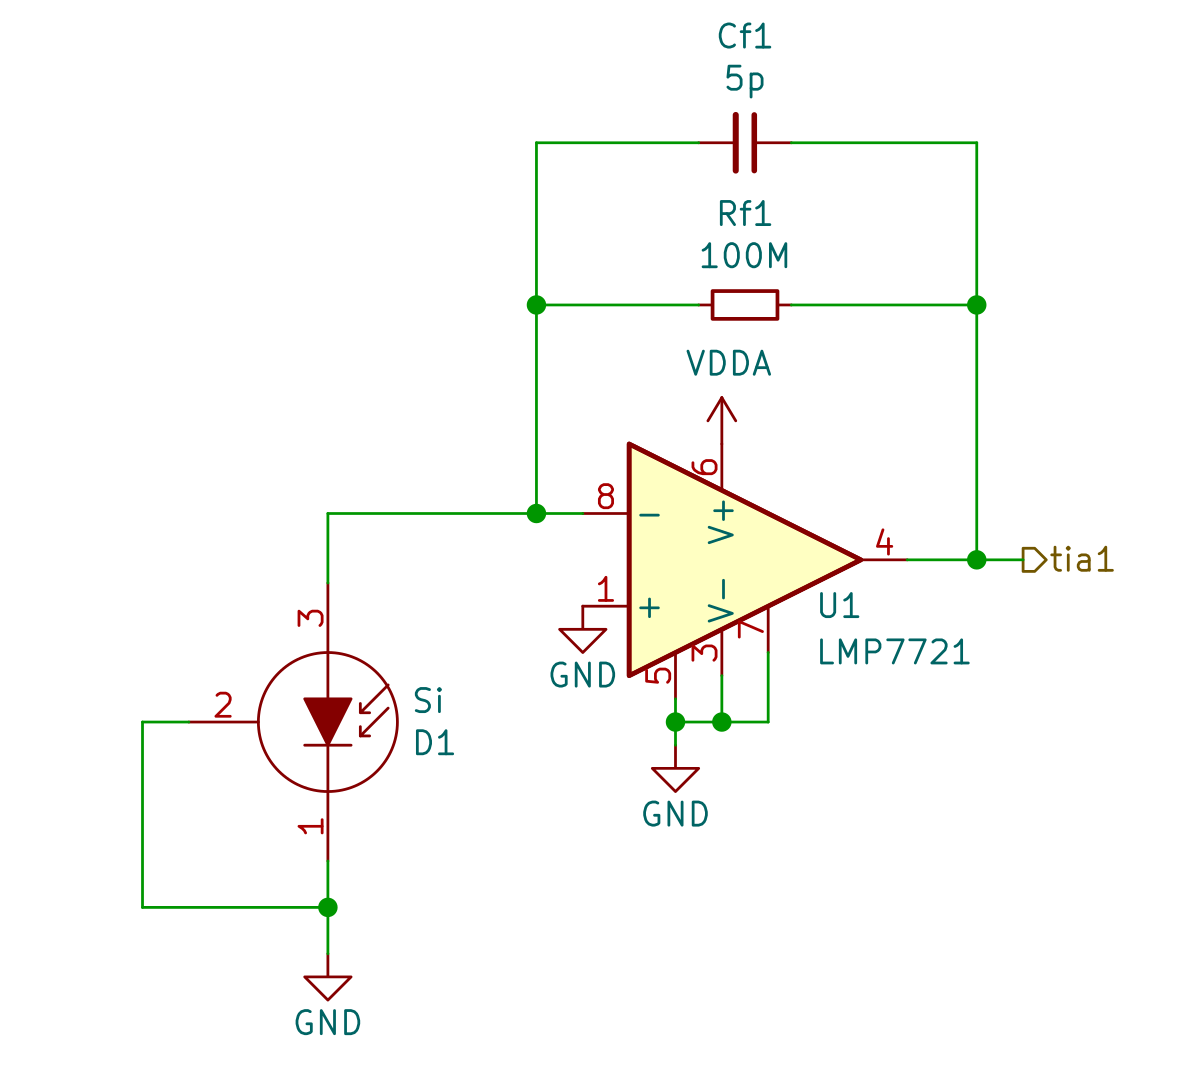
\includegraphics[height=7cm]{slike/fotosenzor.png}
            \caption{Električna shema fotodetektora}
            \label{fig:fotosenzor}
        \end{figure}

        Izlaz svakog fotodetektora propušta se kroz niskopropusni RC filtar s graničnom frekvencijom 1590 Hz, a zatim se dovodi na ulaz analogno-digitalnog pretvornika ADS131M08. Na pločici se nalaze i tri temperaturna senzora ADT7301 radi prilagodbe rezultata mjerenja s obzirom na temperaturu.
        
        ADC i temperaturni senzori povezani su s PDH računalom jednim SPI sučeljem. Prijenosne linije SPI sučelja, kao i CS linije pojedinih sklopova i drugi upravljački signali, dovedene su do pločice na kojoj se nalazi PDH računalo putem konektora s 40 priključaka, čiji je raspored izvoda prikazan na slici \ref{fig:konektor}.

        \begin{figure}[h]
            \centering
            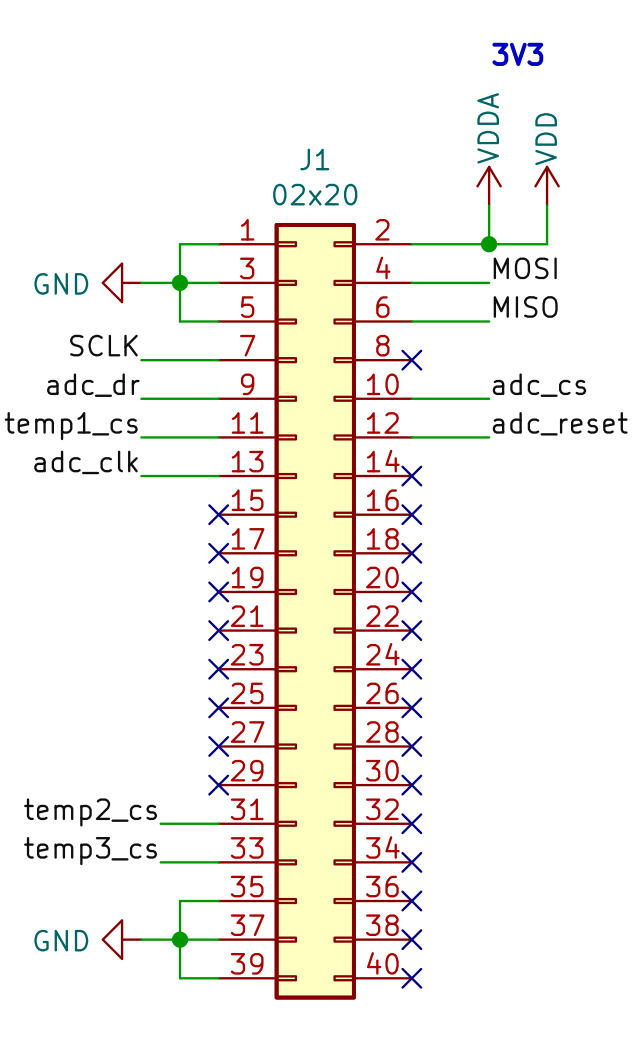
\includegraphics[height=7cm]{slike/konektor.png}
            \caption{Raspored izvoda konektora na senzorskoj pločici}
            \label{fig:konektor}
        \end{figure}

    \section{AD pretvornik ADS131M08}

        \subsection{Opis rada sklopa}
            ADS131M08 je 24-bitni, 8 kanalni delta-sigma analogno-digitalni pretvornik \engl{Analog to Digital Converter, ADC} proizvođača Texas Instruments \cite{ads131m08_datasheet}. Za komunikaciju s mikrokontrolerom koristi SPI sučelje. Svih 8 kanala uzorkuje se istovremeno, a za svaki kanal moguće je postaviti programibilno pojačanje od 1 do 128. Frekvencija uzorkovanja također je programibilna i može iznositi do 32 tisuće uzoraka u sekundi. Slika \ref{fig:adt7301_blok_dijagram} prikazuje blok dijagram sklopa.

            \begin{figure}[htb]
                \centering
                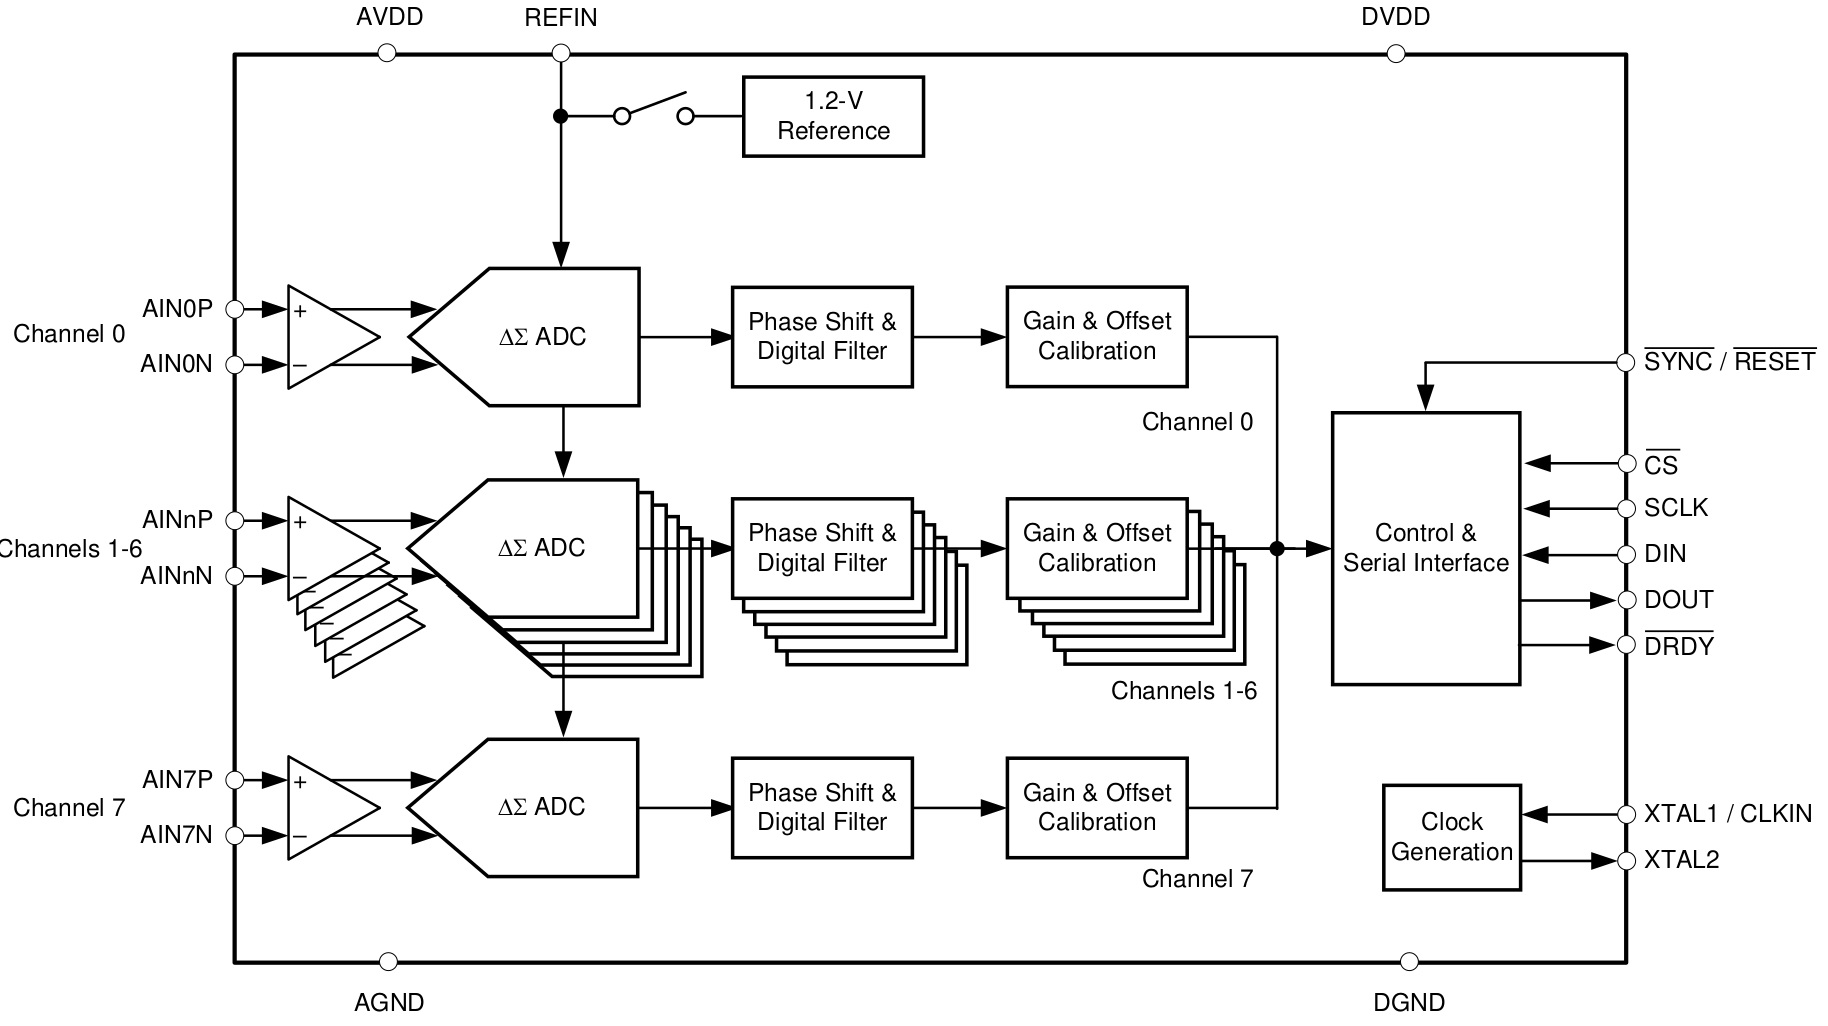
\includegraphics[width=\textwidth]{slike/ads131m08_blok_dijagram.png}
                \caption{Blok dijagram sklopa ADS131M08 \cite{ads131m08_datasheet}}
                \label{fig:ads131m08_blok_dijagram}
            \end{figure}

            Sklop zahtijeva odvojeno napajanje digitalnog i analognog dijela. Analogno napajanje može biti u rasponu 2.7 - 3.6 V, a digitalno napajanje treba biti 1.8 V ili 3.3 V. Referentni napon može se dovesti na vanjski priključak, ili se može koristiti unutarnji izvor referentnog napona iznosa 1.2 V. Signal takta može se generirati unutar sklopa ili može biti doveden na vanjski priključak. 

        \subsection{SPI sučelje}
            SPI sučelje sklopa ADS131M08 koristi postavke CPOL = 0 i CPHA = 1, što znači da niska logička razina odgovara neaktivnom stanju takta i da se podatak čita na drugi brid takta (padajući). Za komunikaciju se koriste standardni SPI priključci (SCLK, MOSI, MISO i \textoverline{CS}) i dva dodatna priključka: \textoverline{DRDY} (\textit{Data Ready}) i \textoverline{SYNC/RESET}.
            
            \textoverline{DRDY} priključak postaje aktivan u trenutku kada je sklop spreman poslati rezultate konverzije. Aktiviranje priključka može se iskoristiti za okidanje prekida na mikrokontroleru, što omogućuje pravovremeno čitanje. Posebnu pažnju treba obratiti kada se podaci čitaju prvi put nakon uključenja ili kada je prošlo dulje vrijeme od zadnjeg čitanja. Naime, ADC ima unutarnji međuspremnik u kojem se spremaju rezultati konverzije ako nisu pročitani. Međuspremnik ima dovoljno kapaciteta za spremanje posljednje dvije konverzije. Kada je međuspremnik pun, ponašanje priključka \textoverline{DRDY} neće biti dosljedno. Proizvođač zato preporuča dva načina za sinkronizaciju: prvi je pročitati dva uzorka zaredom bez čekanja aktivacije \textoverline{DRDY} priključka i tako isprazniti međuspremnik \cite[str.~40]{ads131m08_datasheet}. Drugi način sinkronizacije je postavljanje pravokutnog impulsa trajanja duljeg od jednog perioda signala takta ADC-a, ali kraćeg od 2048 perioda na priključak \textoverline{SYNC/RESET} \cite[str.~40, 46]{ads131m08_datasheet}.

            Podaci se prenose preko SPI sučelja u takozvanim okvirima. Svaki okvir sastoji se od 10 riječi (ili manje, ako su neki kanali onemogućeni). Duljina riječi može se postaviti na 16, 24 ili 32 bita, a pretpostavljena duljina je 24 bita. Sučelje radi u \textit{Full-Duplex} načinu rada. Vremenski dijagram jednog okvira prikazan je na slici \ref{fig:ads131m08_spi_vremenski_dijagram}.

            \begin{figure}[htb]
                \centering
                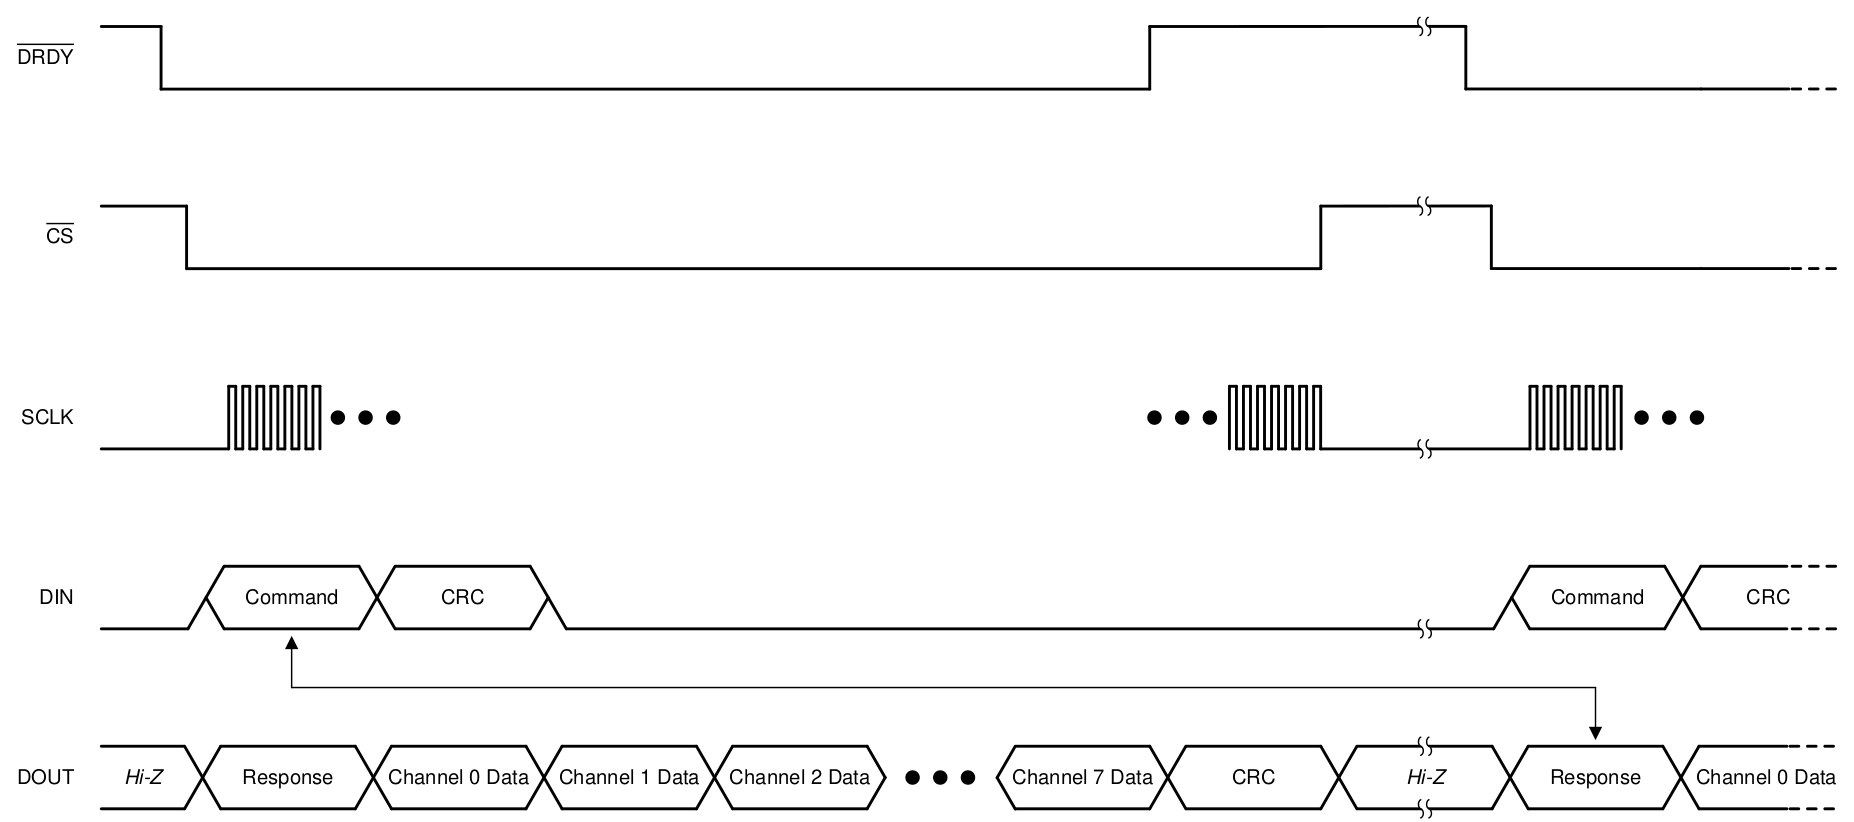
\includegraphics[width=\textwidth]{slike/ads131m08_spi_vremenski_dijagram.png}
                \caption{Vremenski dijagram SPI komunikacije. Strelica označava naredbu i pripadajući odgovor. \cite{ads131m08_datasheet}}
                \label{fig:ads131m08_spi_vremenski_dijagram}
            \end{figure}

            Prva riječ okvira na liniji MOSI (na slici označeno DIN) jest naredba koju \textit{master} uređaj šalje ADC-u. Najčešće korištena naredba je \textit{Null} naredba, čiji je instrukcijski kod 0x0000. Kada primi tu naredbu, ADC neće obaviti nikakvu operaciju, već će samo poslati rezultate konverzije. Neke druge naredbe su RREG (čitanje registra), WREG (upis u registar) i RESET. Druga riječ okvira je CRC (\textit{Cyclic Redundancy Check}) zaštitni kod poruke (ili riječ bitova u niskoj razini ako je CRC onemogućen), nakon čega slijedi 8 riječi s bitovima u niskoj logičkoj razini.

            Prva riječ okvira na liniji MISO (na slici označeno DOUT) jest odgovor na naredbu u prethodnom okviru. Ako je naredba bila \textit{Null}, tada je odgovor ispis sadržaja registra stanja ADC-a. U slučaju neke druge naredbe odgovor se može sastojati i od više riječi, na primjer ako se radi o ispisu sadržaja nekoliko registara. Nakon odgovora slijedi 8 riječi, po jedna za svaki kanal, koje sadrže rezultate AD pretvorbe. Moguće je onemogućiti neke kanale korištenjem naredbe WREG, u tom će slučaju riječ koja odgovara tom kanalu biti izostavljena. Posljednja riječ u okviru je CRC zaštitni kod poruke.
            
    \section{Temperaturni senzor ADT7301}

        \subsection{Opis rada sklopa}
            Sklop ADT7301 proizvođača Analog Devices je temperaturni senzor s integriranim 13-bitnim analogno-digitalnim pretvornikom i serijskim sučeljem SPI. Omogućuje mjerenje temperature u rasponu od -40\textcelsius{} do 150\textcelsius{}, s rezolucijom 0.03125\textcelsius{} i tipičnom preciznošću \textpm{} 0.5\textcelsius{} \cite{adt7301_datasheet}. Blok dijagram sklopa prikazan je na slici \ref{fig:adt7301_blok_dijagram}.
            
            \begin{figure}[htb]
                \centering
                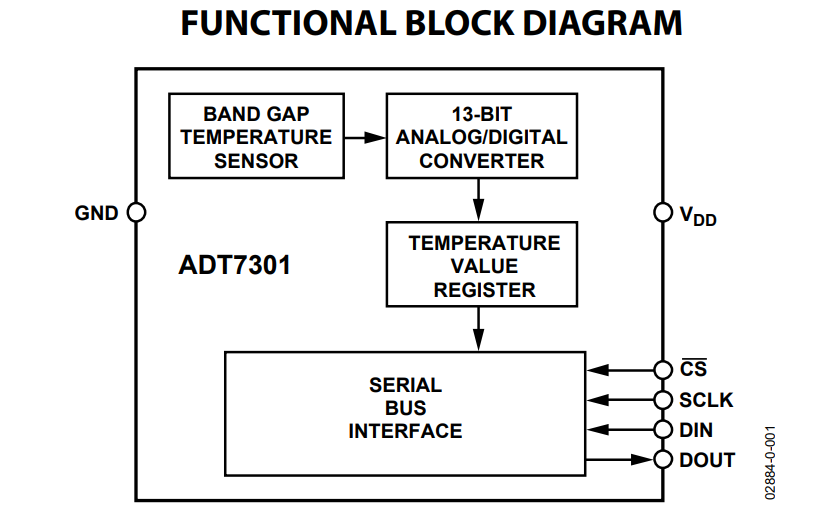
\includegraphics{slike/ADT7301_blok_dijagram.png}
                \caption{Blok dijagram sklopa ADT7301 \cite{adt7301_datasheet}}
                \label{fig:adt7301_blok_dijagram}
            \end{figure}

            Senzor uzima mjerenja temperature svakih 1.5 sekundi, što je regulirano internim sklopom za mjerenje vremena \engl{timer}. Između dva mjerenja, napajanje analognog sklopovlja senzora je ugašeno te ono postaje neaktivno. Digitalno sklopovlje uvijek je aktivno, ali ako se pokuša pročitati vrijednost temperature više puta unutar jednog intervala mjerenja senzor će uvijek vraćati istu vrijednost (onu koju je izmjerio na početku intervala).
            
            Dodatna mogućnost sklopa je takozvani \textit{shutdown} način rada. U ovom načinu rada sklop troši vrlo malo struje (oko 1 \textmu{}A), što je korisno ako postoji dulje vremensko razdoblje u kojem se neće uzimati uzorci temperature. \textit{Shutdown} način rada omogućuje se upisom odgovarajućeg bita u kontrolni registar putem serijskog sučelja.
            
            Prilikom ispitivanja senzora u uvjetima sobne temperature, primijećeno je kako nakon nekoliko minuta kontinuiranog rada očitana temperatura počinje rasti, te može pokazivati vrijednosti čak i do 55\textcelsius{}. Zaključeno je da je navedeno posljedica zagrijavanja samog senzora. Zato je odlučeno da će se senzor između mjerenja stavljati u \textit{shutdown} način rada, kako bi se smanjila potrošnja struje, i samim time disipacija toplinske energije.

        \subsection{SPI sučelje}
            Temperaturni senzor ADT7301 koristi SPI postavke CPOL = 1 i CPHA = 1, što znači da visoka logička razina signala takta odgovara neaktivnom stanju i da se podatak čita na drugi brid takta (rastući).
            
            ADT7301 u stanju je istovremeno slati i primati podatke \engl{Full Duplex}. Na svojem priključku DOUT, koji je spojen na SPI liniju MOSI, sklop daje 16-bitni izlazni podatak na način da najznačajniji bit podatka izlazi prvi. Bitovi 15 i 14 su u niskoj logičkoj razini, bit 13 je bit predznaka, a ostali bitovi predstavljaju apsolutnu vrijednost očitane temperature. Na priključku DIN, koji je spojen na SPI liniju MISO, sklop prima 16-bitni podatak, gdje svi bitovi osim trećeg najznačajnijeg bita moraju biti u niskoj logičkoj razini. Treći najznačajniji bit je 1 u slučaju da se sklop želi staviti u \textit{shutdown} način rada nakon završetka ciklusa slanja, a 0 inače. Slika \ref{fig:adt7301_spi} prikazuje jedan SPI ciklus čitanja/pisanja.
            
            \begin{figure}[htb]
                \centering
                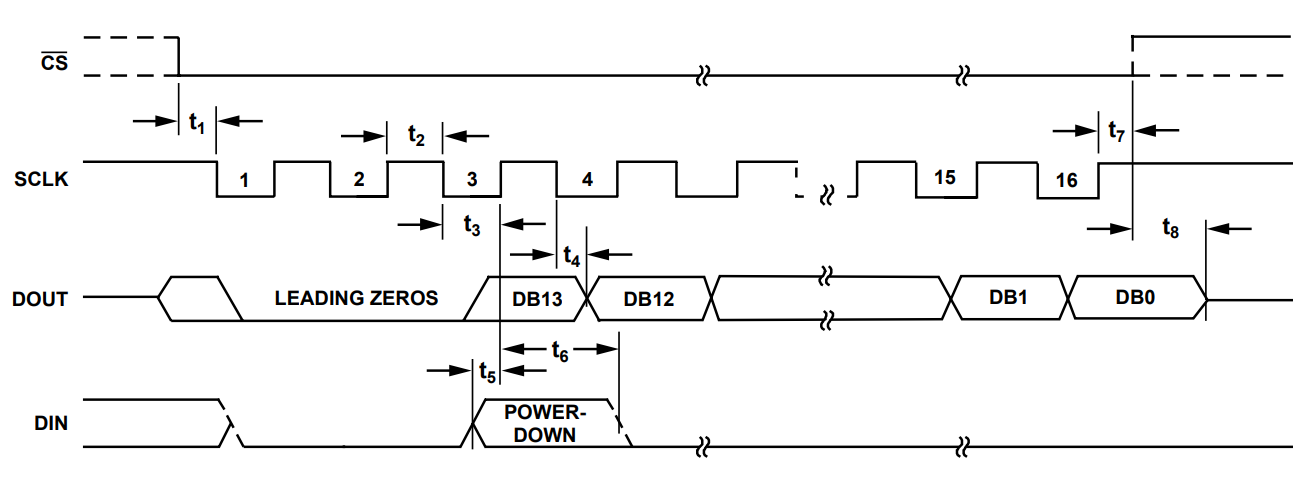
\includegraphics[width=\textwidth]{slike/ADT7301_spi.png}
                \caption{Vremenski dijagram SPI komunikacije sklopa ADT7301 \cite{adt7301_datasheet}}
                \label{fig:adt7301_spi}
            \end{figure}
                